\chapter{Rozszerzenia modelu i dodatkowe konfiguracje}\label{chap:extensions}

W tym rozdziale przeanalizowano dodatkowe konfiguracje licencyjne rozszerzające bazowy model. W szczególności rozważono:
\begin{itemize}
  \item warianty \texttt{roman\_domination} o parametrach cenowych $p\in\{1{,}5,2{,}0,2{,}5,3{,}0\}$ (oznaczenia \texttt{roman\_p\_x}),
  \item konfigurację \texttt{spotify} obejmującą licencje \emph{Individual}, \emph{Duo} (dokładnie 2 osoby) i \emph{Family} (grupa rodzinna),
  \item porównanie z bazową \texttt{duolingo\_super}.
\end{itemize}

\paragraph{Dane i ograniczenia} Analiza wykorzystuje istniejące wyniki z folderu \texttt{runs/}: zestawy \texttt{benchmark\_all} (instancje syntetyczne, scenariusz statyczny) oraz \texttt{dynamic\_20} i \texttt{20250907\_014311\_dynamic} (scenariusz dynamiczny). Część \texttt{dynamic\_real} nie została jeszcze ukończona i nie jest tu używana. W obecnych wynikach nie ma wariantów \texttt{duolingo\_super} innych niż konfiguracja bazowa. Graf \texttt{tree} nie był dotąd uruchamiany w rozszerzeniach i nie jest raportowany.

\section{Metodyka}

Do przygotowania wykresów i zestawień użyto skryptu \texttt{scripts/analysis/model\_extensions.py}, który:
\begin{itemize}
  \item agreguje \textit{cost per node} oraz \textit{time [ms]} per algorytm dla wskazanych konfiguracji,
  \item rysuje porównania grupowe (słupki) między wieloma konfiguracjami,
  \item w przypadku \texttt{roman\_p\_x} tworzy krzywą kosztu w funkcji parametru $p$ dla każdego algorytmu,
  \item wylicza i wizualizuje miks typów licencji (udziały) dla konfiguracji \texttt{spotify}.
\end{itemize}
Wykresy zapisano w \texttt{docs/thesis/assets/figures/extensions/}.

\section{Warianty roman\_p\_x}

Rysunek \ref{fig:roman_group} pokazuje porównanie średniego \textit{cost per node} oraz \textit{time [ms]} (uśrednienie po instancjach) dla algorytmów i pięciu konfiguracji: \texttt{roman\_domination}, \texttt{roman\_p\_1\_5}, \texttt{roman\_p\_2\_0}, \texttt{roman\_p\_2\_5}, \texttt{roman\_p\_3\_0}. Rysunek \ref{fig:roman_curve} prezentuje zależność kosztu od parametru $p$ (krzywe per algorytm).

\begin{figure}[H]
  \centering
  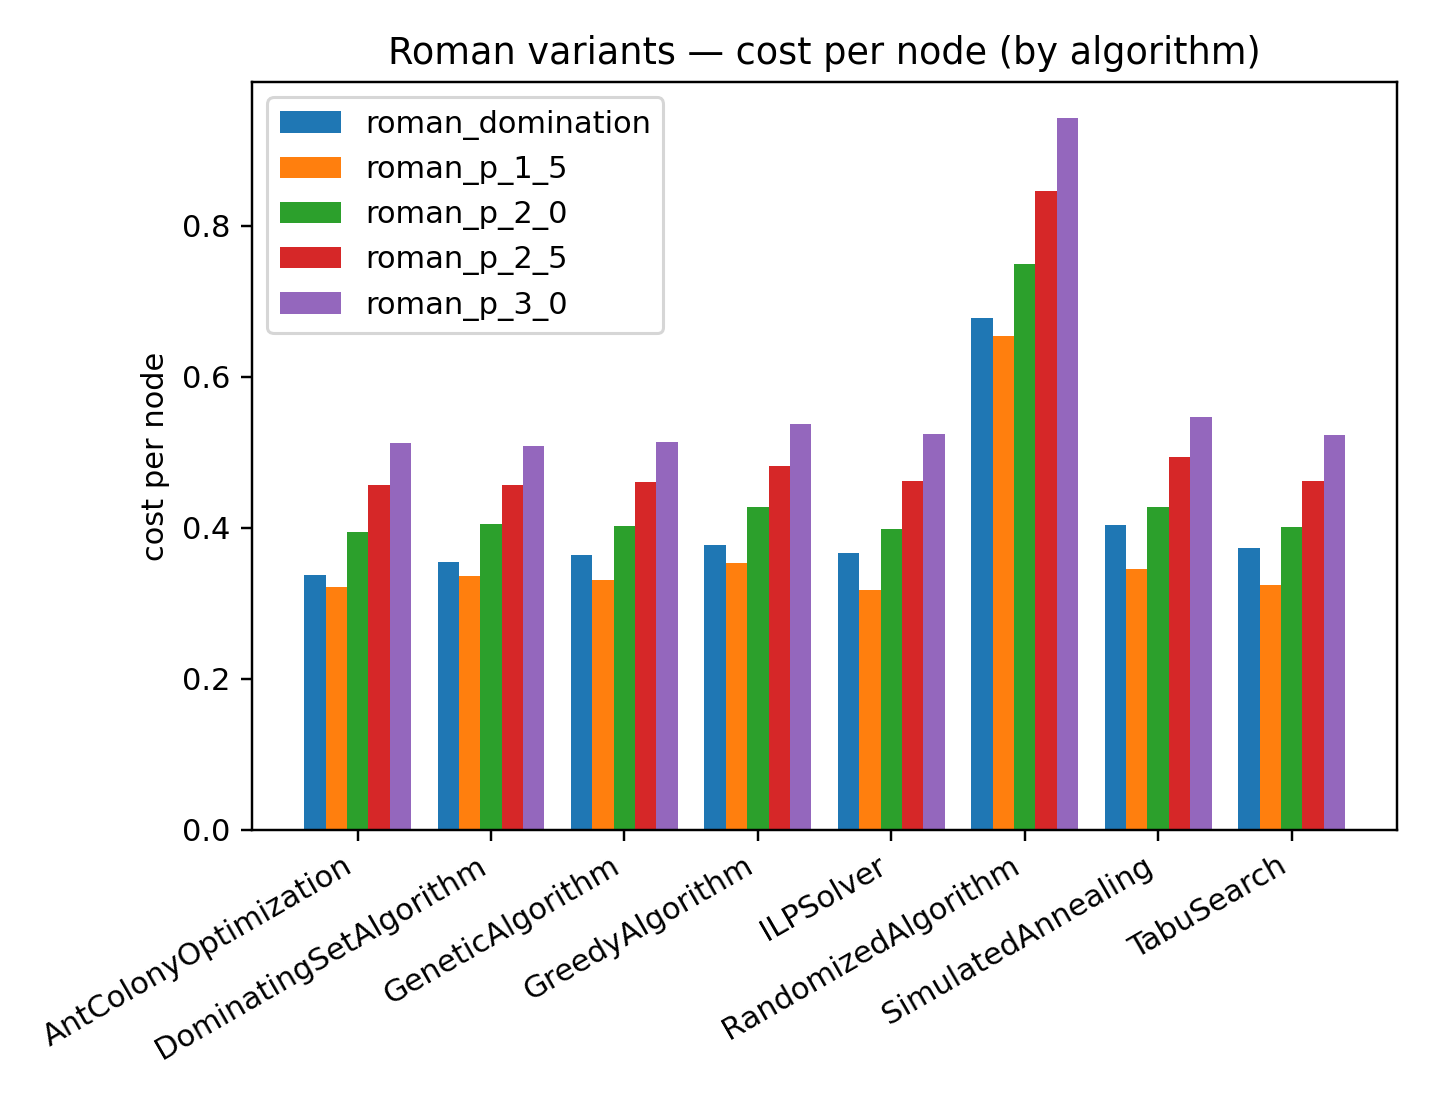
\includegraphics[width=0.48\linewidth]{assets/figures/extensions/roman_variants_cost.png}
  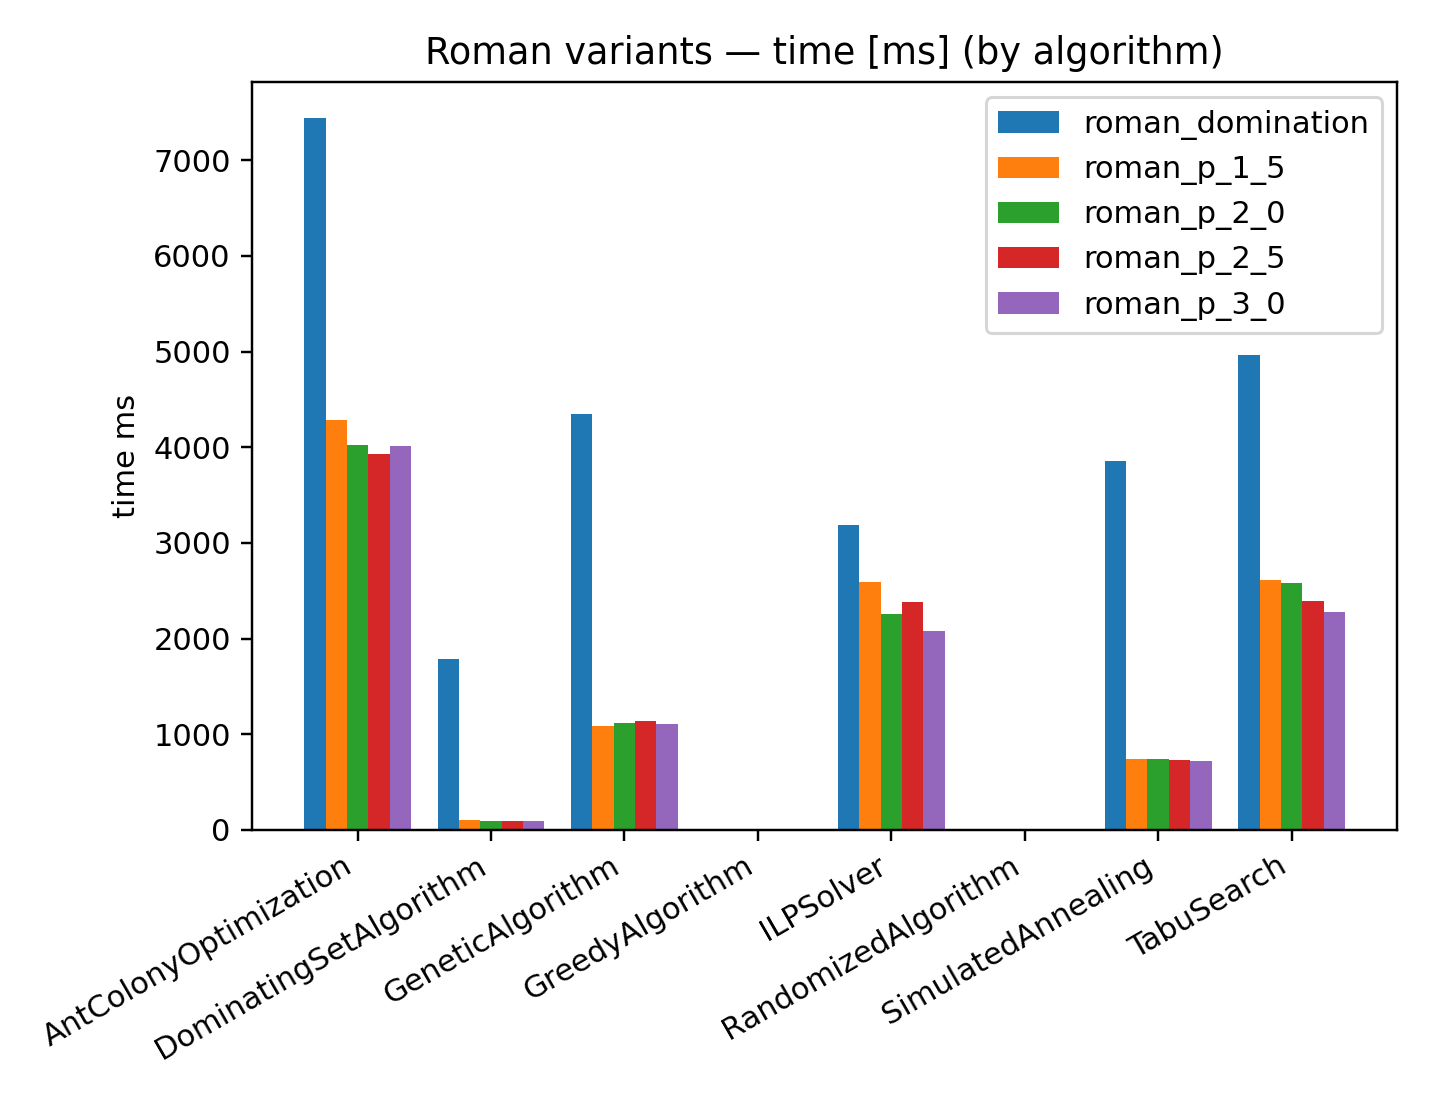
\includegraphics[width=0.48\linewidth]{assets/figures/extensions/roman_variants_time.png}
\caption{Warianty roman\_p\_x: koszt na wierzchołek i czas działania (per algorytm).}
  \label{fig:roman_group}
\end{figure}

\begin{figure}[H]
  \centering
  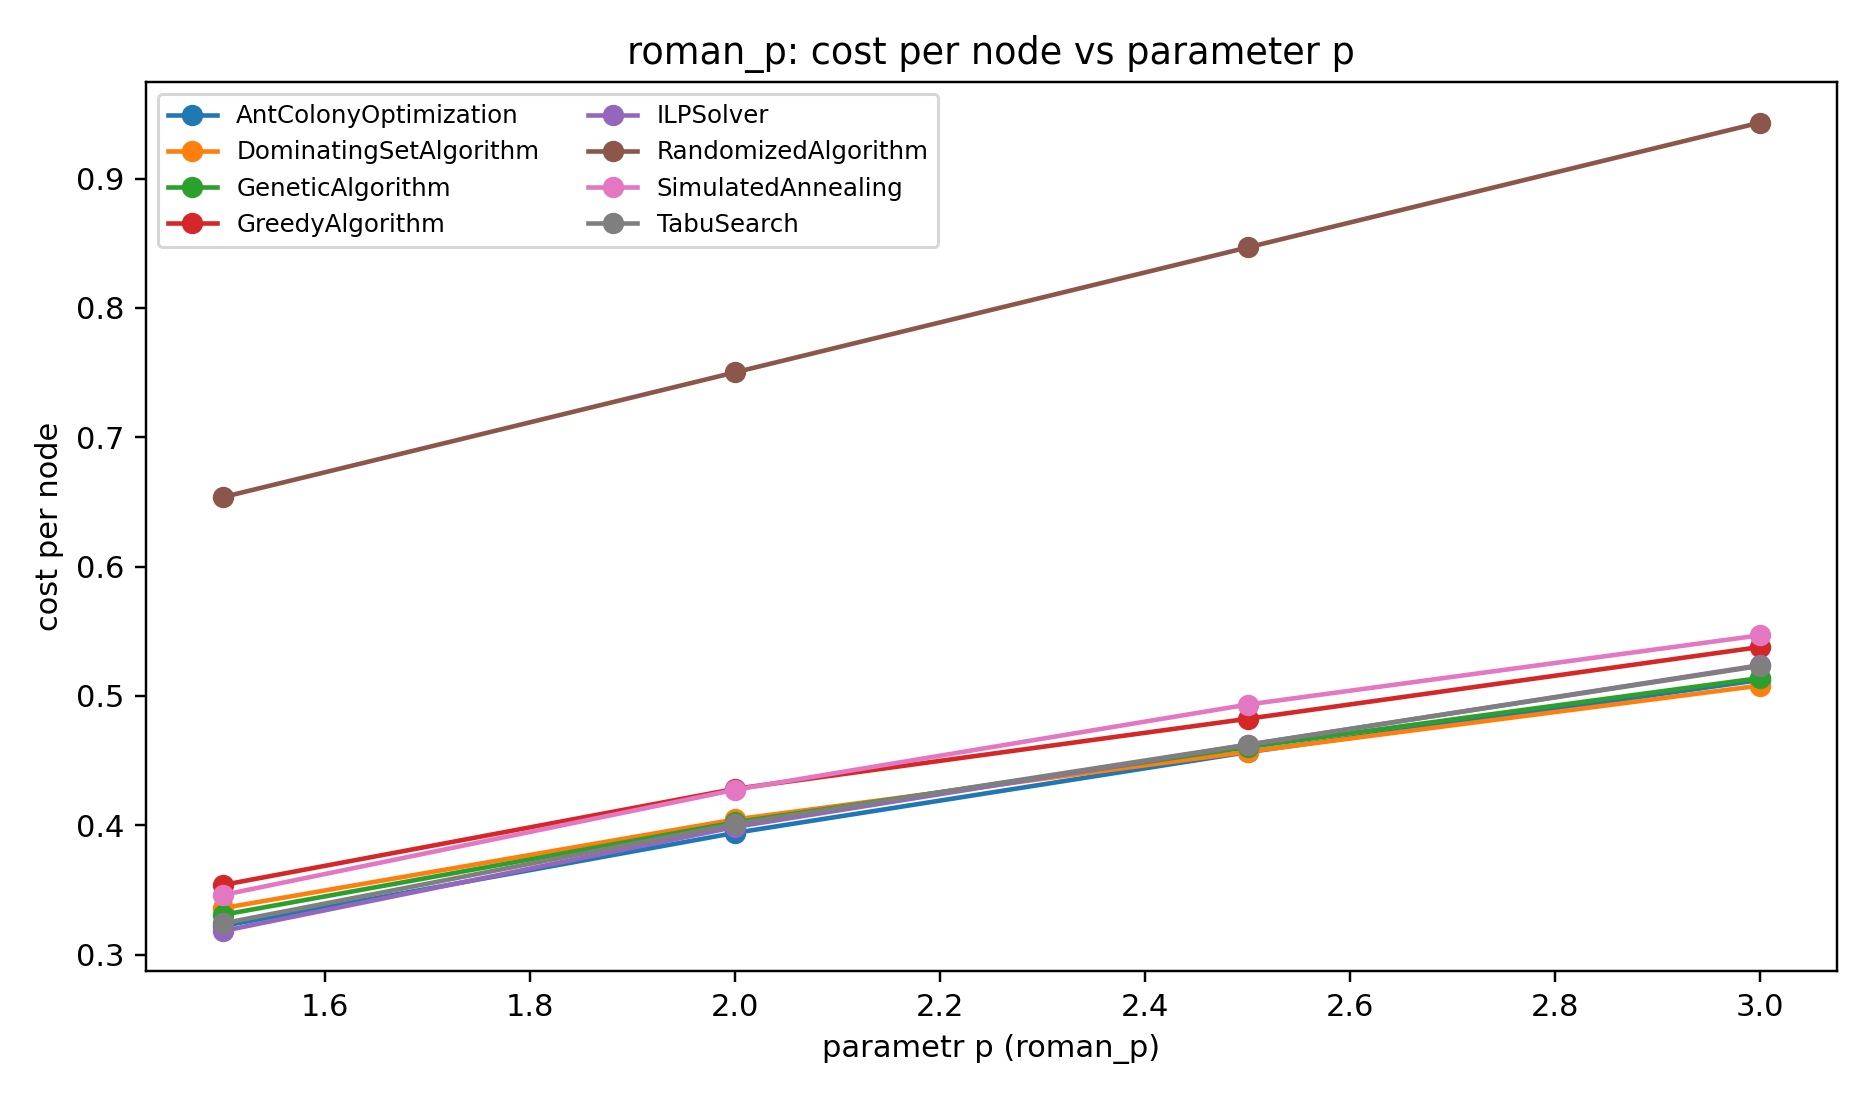
\includegraphics[width=0.7\linewidth]{assets/figures/extensions/roman_p_curve_cost_per_node.png}
\caption{roman\_p\_x: koszt na wierzchołek vs parametr $p$ (krzywe per algorytm).}
  \label{fig:roman_curve}
\end{figure}

\paragraph{Wyniki i obserwacje}
Zgodnie z intuicją, wzrost parametru cenowego $p$ powoduje wzrost kosztu na wierzchołek w całym przekroju algorytmów. Mediana \textit{cost per node} (z \texttt{benchmark\_all}) dla wybranych wariantów kształtuje się przykładowo następująco: \texttt{roman\_p\_1\_5} $\approx0{,}308$, \texttt{roman\_p\_2\_0} $\approx0{,}400$, \texttt{roman\_p\_2\_5} $\approx0{,}476$, \texttt{roman\_p\_3\_0} $\approx0{,}537$. Różnice między algorytmami pozostają podobne do obserwacji z części statycznej: metaheurystyki uzyskują niższe koszty, kosztem dłuższego czasu obliczeń, podczas gdy heurystyki konstrukcyjne (zachłanny, dominating set) są szybsze, lecz nieco droższe.

\section{Konfiguracja Spotify i porównanie z Duolingo Super}

Konfiguracja \texttt{spotify} obejmuje trzy typy licencji: \emph{Individual}, \emph{Duo} (dokładnie 2 osoby) i \emph{Family}. Rysunek \ref{fig:duo_spotify_cmp} porównuje \textit{cost per node} oraz \textit{time [ms]} między \texttt{spotify} a \texttt{duolingo\_super}. Na rysunku \ref{fig:spotify_mix} pokazano miks licencji (udział typów) per algorytm.

\begin{figure}[H]
  \centering
  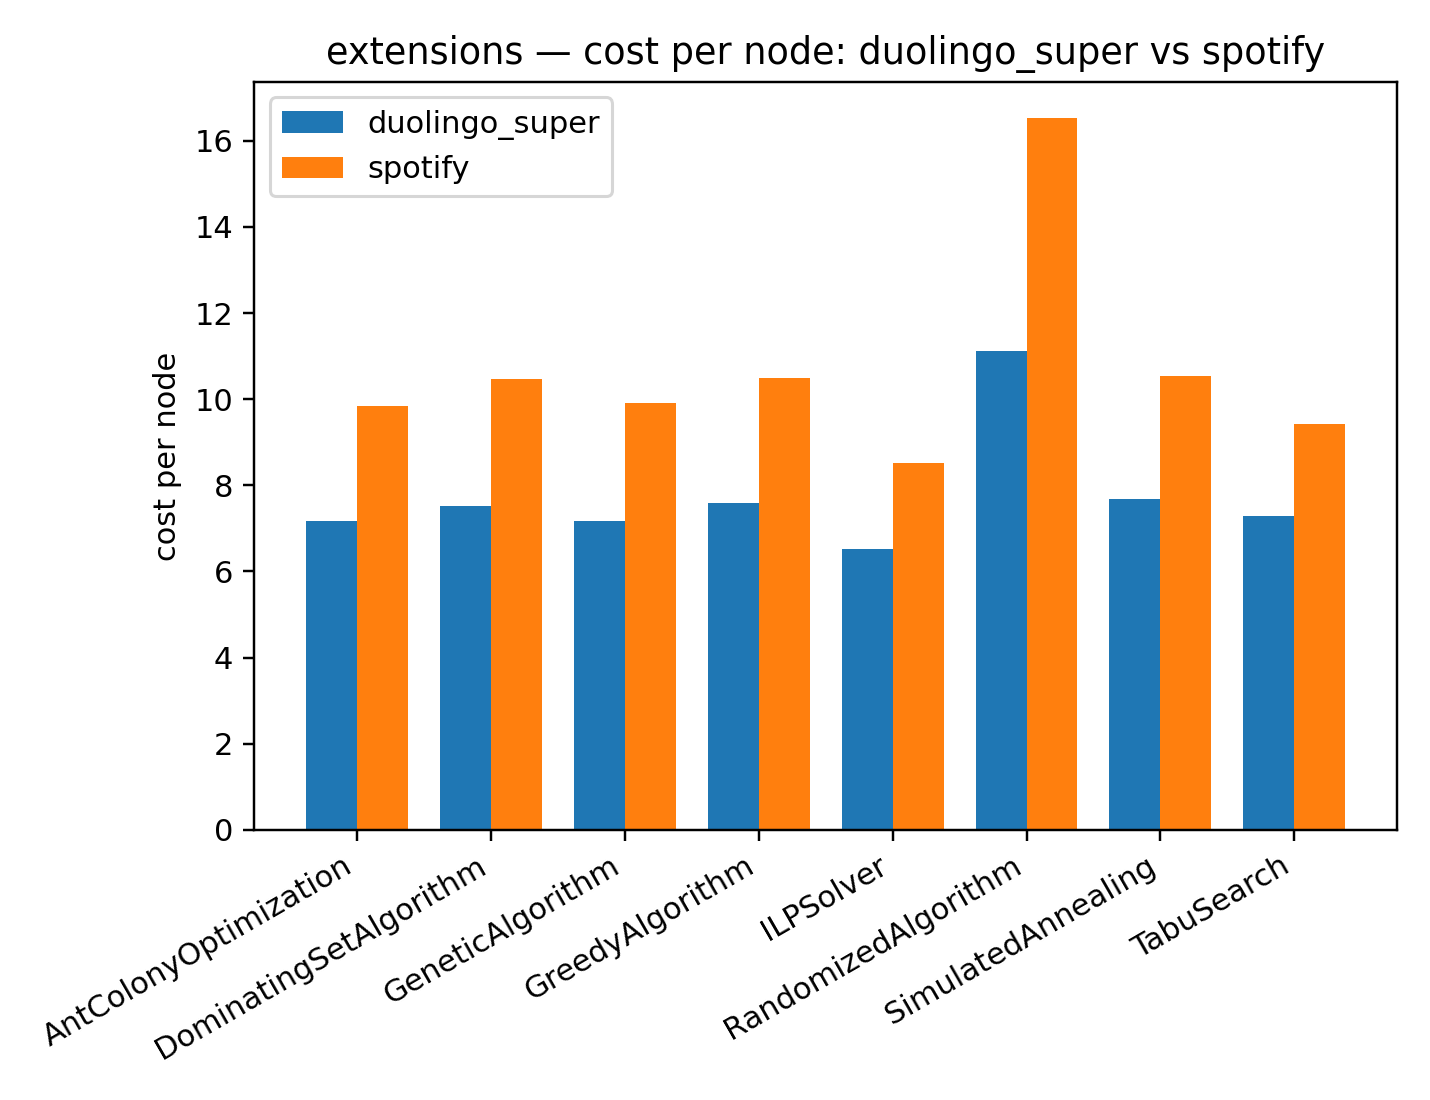
\includegraphics[width=0.48\linewidth]{assets/figures/extensions/duo_vs_spotify/compare_cost_per_node_duolingo_super_vs_spotify.png}
  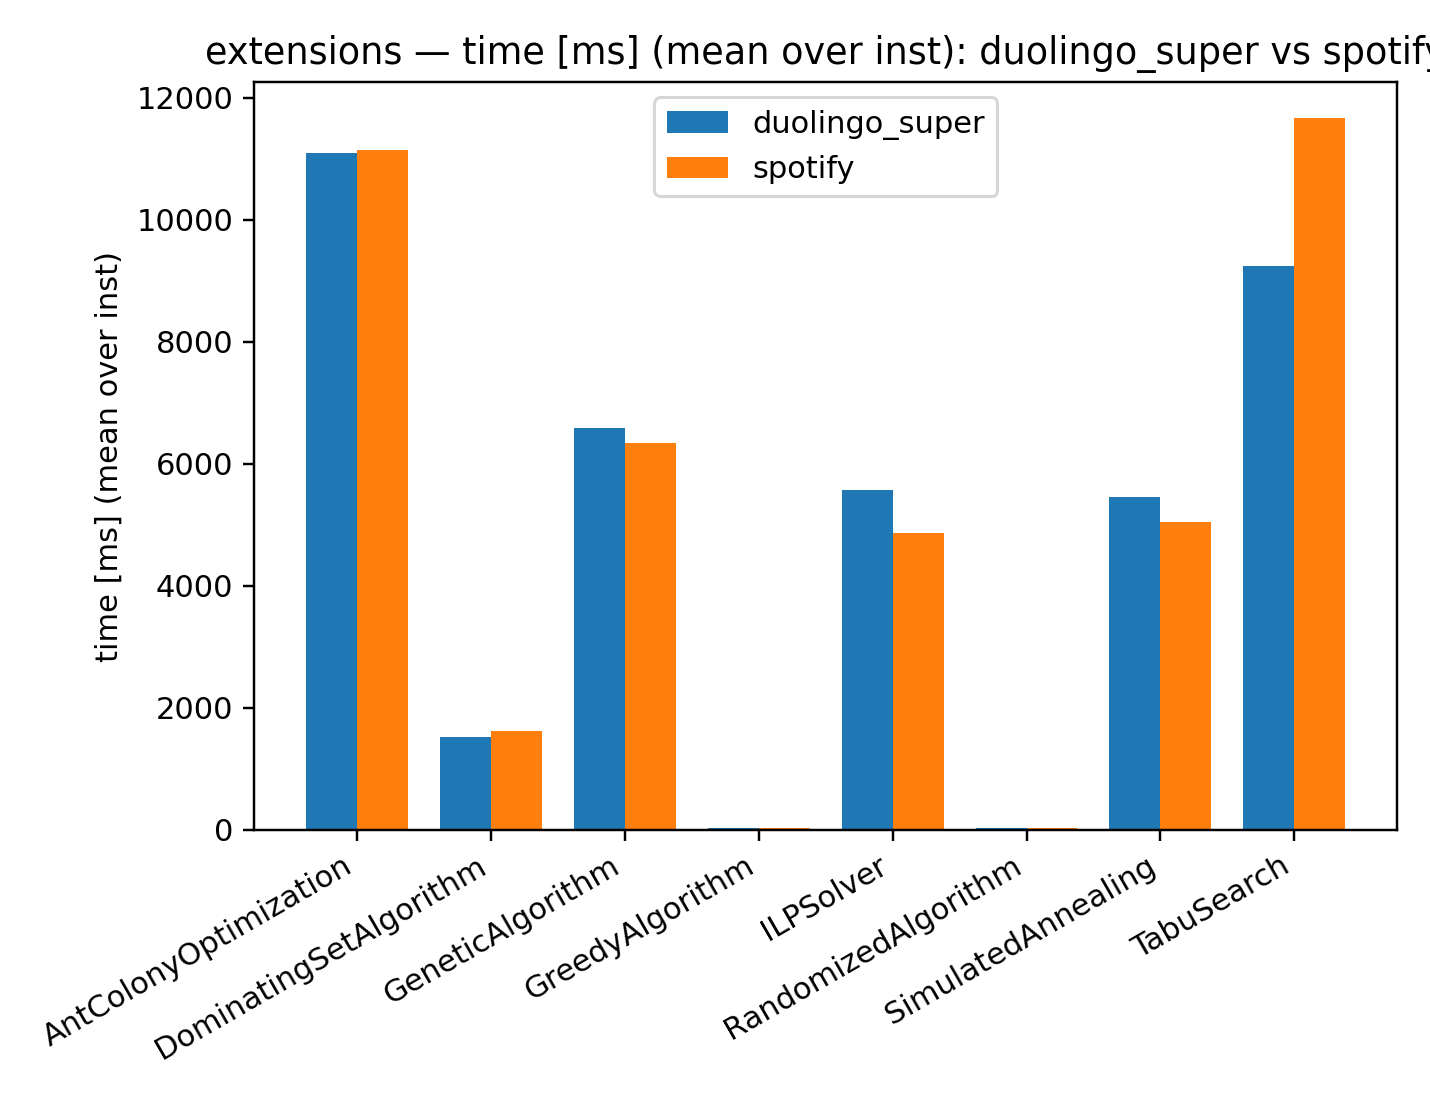
\includegraphics[width=0.48\linewidth]{assets/figures/extensions/duo_vs_spotify/compare_time_ms_duolingo_super_vs_spotify.png}
\caption{Porównanie Duolingo Super vs Spotify: koszt na wierzchołek i czas (średnio per algorytm).}
  \label{fig:duo_spotify_cmp}
\end{figure}

\begin{figure}[H]
  \centering
  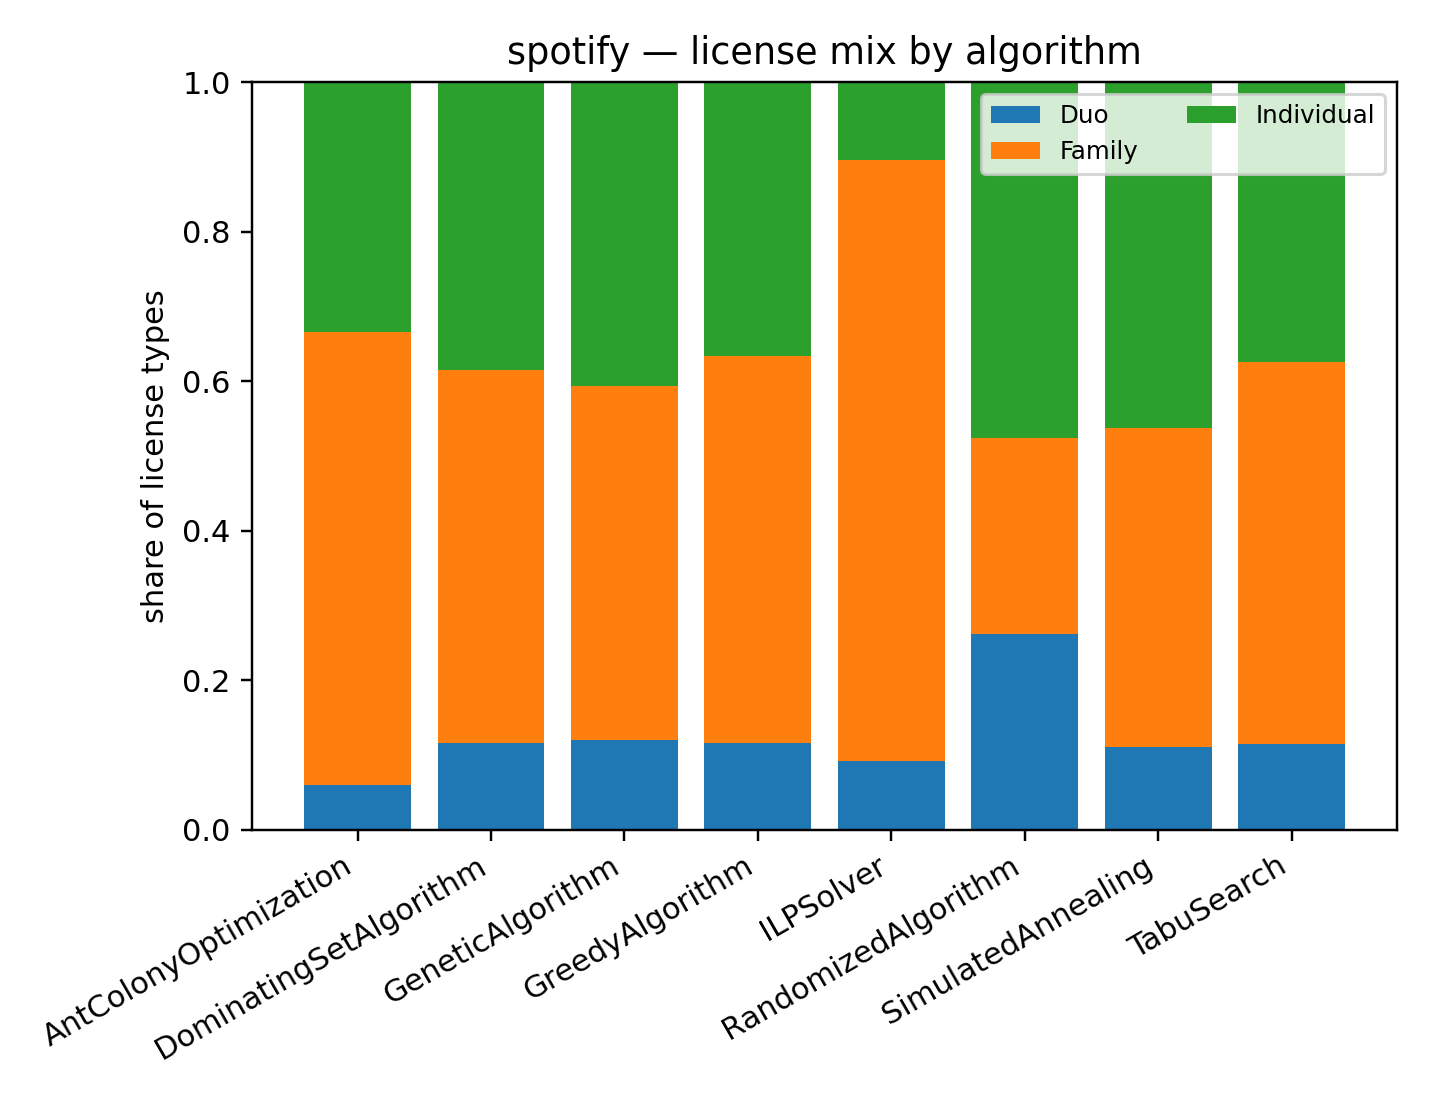
\includegraphics[width=0.75\linewidth]{assets/figures/extensions/spotify_license_mix.png}
\caption{Spotify: udziały typów licencji per algorytm (Individual/Duo/Family).}
  \label{fig:spotify_mix}
\end{figure}

\paragraph{Wyniki i interpretacja}
W przekroju instancji syntetycznych (\texttt{benchmark\_all}) mediana \textit{cost per node} dla \texttt{duolingo\_super} wynosi około $6{,}81$, natomiast dla \texttt{spotify} około $8{,}95$. Wyższy koszt w \texttt{spotify} wynika z inaczej ukształtowanego cennika oraz dodatkowego typu \emph{Duo} ograniczonego do par (brak możliwości dalszego skalowania grupy). Udział \emph{Duo} zależy od algorytmu: dla metod konstrukcyjnych i metaheurystyk typowo 10–12\%, zaś dla algorytmu losowego sięga około 26\%. Z kolei \emph{Family} dominuje w rozwiązaniach ILP (ok. 86\%), co wskazuje, że przy sprzyjającej strukturze grafu optymalne jest formowanie większych grup rodzinnych. Czas obliczeń jest porównywalny między konfiguracjami, zależny głównie od wybranego algorytmu oraz rozmiaru/gęstości grafu.

\section{Uwaga o wariantach \texttt{duolingo\_super}}

W aktualnym zestawie wyników brak uruchomień wariantów \texttt{duolingo\_super} innych niż konfiguracja bazowa. W przypadku dodania alternatywnych parametrów (np. zmienione progi pojemności i ceny), proponuje się powtórzyć powyższą procedurę porównawczą: porównania grupowe (koszt/czas per algorytm), wykresy miksu licencji oraz – w scenariuszu dynamicznym – trajektorie kosztu w czasie z rozróżnieniem warm/cold (jeśli dostępne).

\section{Wnioski}

\begin{itemize}
  \item Warianty \texttt{roman\_p\_x} wykazują monotoniczny wzrost kosztu wraz ze wzrostem parametru $p$, zgodnie z oczekiwaniami; relatywna przewaga algorytmów pozostaje zbliżona do obserwacji z części statycznej.
  \item Konfiguracja \texttt{spotify} jest średnio droższa na wierzchołek niż \texttt{duolingo\_super}, co wynika z obecności licencji \emph{Duo} (para) i innej struktury cenowej; przy strukturach grafu sprzyjających większym grupom przewagę kosztową zapewnia \emph{Family}.
  \item Brak wariantów \texttt{duolingo\_super} w obecnych wynikach ogranicza porównania; po ich dodaniu rekomenduje się analogiczną analizę jak dla \texttt{roman\_p\_x} i \texttt{spotify}.
\end{itemize}
